\documentclass[12pt, DIV=12]{scrartcl}

% Use the modern KOMA package for headers and footers
\usepackage[automark, headsepline=0.4pt]{scrlayer-scrpage}

\usepackage[utf8]{inputenc}      % SELBST HINZUGEFÜGT
\usepackage{float}				 % Figure im Text verankern können
\usepackage[pdftex]{graphics}    % Einbinden von Bildern 
\usepackage{graphicx}            % Einbinden von Bildern (jpg)
\usepackage{amsmath}             % Mathematical Society Package
\usepackage[bf]{caption}         % Bildunterschriftenformatierung
\usepackage{siunitx} 			 % SI Einheiten
\usepackage{subcaption} % For subfigures



\sisetup{separate-uncertainty=true,exponent-product = \cdot,} % durch diese Parameter wird bewirkt, dass Fehlerangaben in der von uns bevorzugten Weise erfolgen, also (Wert +- Fehler) Einheit

\usepackage[automark, headsepline=0.4pt]{scrlayer-scrpage}	 % Spezielle Kopf- und Fußzeilen; automark=automatische Aktualisierung der Kapitel
\usepackage{color}
\usepackage{fancybox}	% Farben z.B. für Textboxen
\usepackage[colorlinks,	% Farben der Links -> werden dann mit \url{}
			linkcolor=blue,
			urlcolor=blue]{hyperref}
\usepackage{multicol}
\usepackage{amsmath}
\usepackage{upgreek}
\usepackage{microtype}

% Verwenden des Fonts Source Sans 
\usepackage[default,semibold,light]{sourcesans}
\usepackage[T1]{fontenc}

\renewcommand{\title}{On the construction and magnetic response of ellipsoidal raspberry particles} % Titel der Arbeit
\newcommand{\akademischegrade}{}            % bereits erlangte akademische Grade!
\renewcommand{\author}{Florian Christopher Klee}      % Titel Vor Vorname Nachname, Titel Nach
\newcommand{\matrikelnummer}{12124153}      % Matrikelnummer
\newcommand{\studienkennzahl}{UA 066 876}                % Studienkennzahl
\newcommand{\studienrichtung}{Masterstudium
Physics}    % Studienrichtung
\newcommand{\supervisor}{Pedro Antonio Sanchez Romero, PhD}        % BetreuerIn


\setlength{\parindent}{0cm}	% Absätze statt Einrückung Zeilenabstand -> das ist allerdings reine Geschmacksache; Man kann den befehl auch weglassen, dann werden die default Einstellungen genommen
\setlength{\parskip}{0.5cm}                       

\restylefloat{figure}	% Dieser Befehl gilt für alle Gleitumgebungen (float) -> Bilder. Aktivierung des \usepackage{float} 

\ohead{\headmark}	% Kopfzeile - Achtung bei zweiseitigem Layout
\chead{}
\ihead{}											

\ofoot[\pagemark]{\pagemark}
\cfoot{}	%Fußzeile, zentriert
\ifoot{}

\pagestyle{empty}



\begin{document} % Beginn des Dokuments
%TITELSEITE-----------------------------------------------------------
\thispagestyle{empty}

\vspace*{-3.5cm}

\begin{flushright}
    \advance\rightskip-1.5cm
    
\includegraphics[width=7.5cm]{./images/Uni_Logo.png}
\end{flushright}

\vspace{0.5cm}
\begin{center}

    \huge
    \textbf{Project report}

    \vspace{0.1cm}
    \Large in 260035 LP Laboratory: Computational Statistical Mechanics
    \vspace{1cm}

    Titel \textbar{} Title
    \vspace{-0.5cm}

    \Large \title
    \vspace{1.5cm}

    \normalsize
    verfasst von \textbar{}  submitted by

    \vspace{-0.5cm}
    \large \akademischegrade\ \author
    \vspace{0.5cm}

    \normalsize
    betreut von \textbar{} supervised by

    \vspace{-0.5cm}
    \large \akademischegrade\ \supervisor
    \vspace{0.5cm}

    \vspace{1cm}
\end{center}

\begin{flushleft}
    \normalsize
    Wien \textbar{} Vienna, \the\year \\
    \vspace{0.8cm}

    \begin{tabular}{p{8cm}l}
        \raggedright Studienkennzahl lt. Studienblatt \textbar{} degree programme code as it appears on the student record sheet: & \studienkennzahl \\
        \raggedright Studienrichtung  lt. Studienblatt \textbar{} degree programme as it appears on the student record sheet:     & \studienrichtung \\
        %\raggedright Dissertationsgebiet  lt. Studienblatt | degree programme as it appears on the student record sheet:                       & \studienrichtung      \\
    \end{tabular}
\end{flushleft}
%\newpage
%\thispagestyle{empty}
%\mbox{}
%----------------------------------------------------------------------------------------------------
\newpage
\thispagestyle{empty}
\begin{abstract}
    \Large{\textbf{Abstract:}}

    \vspace{0.5cm}
    \normalsize
    This report presents work done in the 260035 LP Laboratory: Computational Statistical Mechanics, towards a larger project on recreating, in simulation, the experimental findings on field induced recirculation flows in a dilute magnetic colloid by Queiros Campos et al (2024) \cite{QueirosCampos2024}.

    The report discribes two different methods of creating densly packed raspberry ellipsoid particles, as well as a qualitative analysis of the magnetic behaviour obtained by applying the Thermal Stoner-Wohlfarth model by Mostarac (2025) \cite{Mostarac2025} to them.

    It is shown that the applied methods suitably reproduce the theoretical initial magnetization curve expected for a non-interacting solid and that the influence of several of the ellipsoids' parameters, qualitatively matches the expected effects on their hystereses.
\end{abstract}

%-------------------------------------------------------------------------------
\newpage
\addtocontents{toc}{\protect\thispagestyle{empty}}
\tableofcontents	% Inhaltsverzeichnis

%-----------------------------------------------------------------------------------
\newpage
\pagestyle{scrheadings}

\section{Introduction}

\subsection{Motivation}

Colloidal motors reffer to systems in which colloidal particles, that is, particles stably dispersed in a carrier medium, are able to travel in a directional manner \cite{Chen2019}.\\
Treatment of blood clots via thrombolytric drug delivery, has the problem that in the vicinity of a blood clot, there is little flow, by which to efficiently deliver the drug. One proposed method to improve this treatment is to use magnetic coloidal motors achived by a rotating magnetic field to induce a recirculation flow in the vicinity, in order to aid the diffusion of the drug or even mechanically erode the clot \cite{Cheng2014}.

\subsection{Studied System}

The system of interest is an experimental setup, shown in Figure \ref{fig_system}, that achieves a recirculation flow in a closed fluid channel. Simplified, the system is initially composed of a water based solution inside a channel of width 1 mm in which maghemite nanoparticles ($\sim 20$ nm) and some primary aggregates of them ($\sim 120-140$ nm) are dispersed.\\
A magnetic field is applied, with a gradient in y direction and a rotating component. The rotating field leads to secondary aggregation into the visible rod shaped structures which spin synchronously with the field, while the field gradient causes the spinning rods to translate towards the back wall and thus produces the visible gradient in their concentration.\\
The paper goes on to describe how the spinning rods excert a rightward force on the back wall (and adjacent fluid), and therefore experience a net force and translation to the left.\\
As a result, the fluid in the region with the aggregates, although disturbed by the rotation, shows a net translation to the left and to counteract this flow in a closed channel, a rightward flow emerges in the front region. The resulting flow profile is show in Figure \ref{fig_flow_profile}.
Some named parameters include, field amplitude $ H_0 =  \mathrm{6.4 \, kA m^{-1}},$ field frequency $f = \mathrm{5 \, Hz}$, volume fraction of particles $ \phi_\mathrm{p} =  \mathrm{3.2 \cdot 10^{-3}}$ and the resulting flow has a characteristic speed of $\sim 5-8 \, \mathrm{\mu m s^{-1}}$. \\

The goal of the overarching project is to emulate this result, by the same mechanisms, in simulation. This report focuses on the creation of analogues to the spinning rod structures and their magnetic response.

\begin{figure}
    \begin{center}
        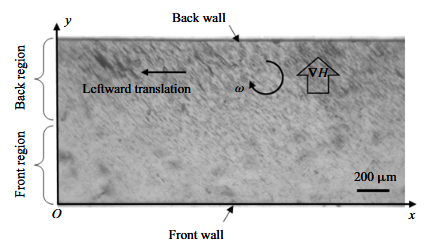
\includegraphics[width=12cm]{./images/System.png}
        \caption{Captured image of channel of carrier fluid with rod shaped colloidal aggregates  co-rotating with magnetic field with frequency $\omega$ and magnetic field gradient $\nabla H$ direction Source: \cite{QueirosCampos2024}.}
        \label{fig_system}

    \end{center}
\end{figure}

\begin{figure}
    \begin{center}
        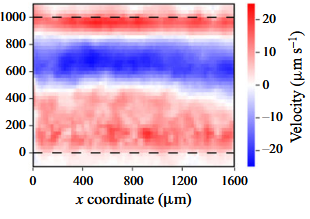
\includegraphics[width=8cm]{./images/flow_profile.png}
        \caption{Induced flow profile in the different regions of the channel, colour coded to demonstrate right vs leftward flowing regions. Source: \cite{QueirosCampos2024}.}
        \label{fig_flow_profile}
    \end{center}
\end{figure}


\section{Models}

\subsection{Raspberry particles}
The rods in the experiment will be modelled in simulation by ellipsoidal raspberry particles with a large semiaxes ratio.\\
Raspberry particles are a rigid arrangement of smaller spherical particles and should serve well to model the multi step aggregates formed in the experiment. Their multi core structure allows for rich magnetic interactions and a structured surface that is well suited to acurately capturing the involved hydrodynamics, while remaining coarse grained enough to be efficient in simulation.\\
Refer to Figure \ref{fig_ell_smooth} for a visual intuition.


\subsection{Weeks-Chandler-Anderson potential}
In finding configurations of particles for different size and shape ellipsoids the Weeks-Chandler-Anderson potential \cite{Weeks1971} is used. It is a modification of the Lennard-Jones potential \cite{LennardJones1931} often used as a continuous approximation for hard sphere particle potentials in molecular dynamics simulations. It takes the following form:

\begin{equation}
    V_\mathrm{WCA}(r) =
    \begin{cases}
        4\epsilon\left[\left(\frac{\sigma}{r}\right)^{12} - \left(\frac{\sigma}{r}\right)^{6}\right] + \epsilon & 0<r<r_\mathrm{cut}                \\
        0                                                                                                       & \hspace{0.75cm}r > r_\mathrm{cut} \\
    \end{cases}
    \label{eqn_WCA}
\end{equation}
with particle distance r, particle diameter $\sigma$, interaction  strength $\epsilon$ and cutoff radius $r_\mathrm{cut} = 2^{1/6} \sigma$.

\subsection{The generalized Stoner-Wohlfarth model}
The implementation of the magnetic interactions of the particles within the ellipsoids is based on the generalized Stoner-Wohlfarth model \cite{Chuev2007} which is introduced here.\\
The original Stoner-Wohlfarth model (SW) \cite{Stoner1948} describes magnetic single domain particles with uniaxial anisotropy, experiencing an external magnetic field. It combines anisotropy energy
\begin{equation}
    E_{\mathrm{ani}} = -K\cos^2(\theta-\phi)
    \label{eqn_ani}
\end{equation}

and Zeeman energy

\begin{equation}
    E_{\mathrm{Zee}} = -M_\mathrm{sat}H\cos\phi
    \label{eqn_zee}
\end{equation}

with anisotropy constant K, saturation magnetization $M_\mathrm{sat}$, angle $\theta$ between applied magnetic field H and the anisotropy axis and angle $\phi$ between the field and the particle's magnetic moment. Figure \ref{fig_SW} shows the geometry, as well as resulting energy density as a function of $\phi$.\\
SW predicts the existence of two energetic minima a magnetic moment can occupy, unless the applied magnetic field exceeds the critical field $H_\mathrm{c}$, in which case only one energetic minimum remains. The model also disregards any transition of state from one minimum to another that doesn't occur because of the disappearance of one of the minima. In the latter case, it is assumed that the magnetic moment instantly transitions to the new minimum.\\
A core result of SW is, that the field required for this transition, for $\theta$ = $45^\circ$, is half the required critical field over the magnetic easy or hard axis. This specific transition is shown in Figure \ref{fig_SW} (right) where for H = 0.5 one minimum vanishes into a saddle point.

\begin{figure}[H]
    \begin{center}
        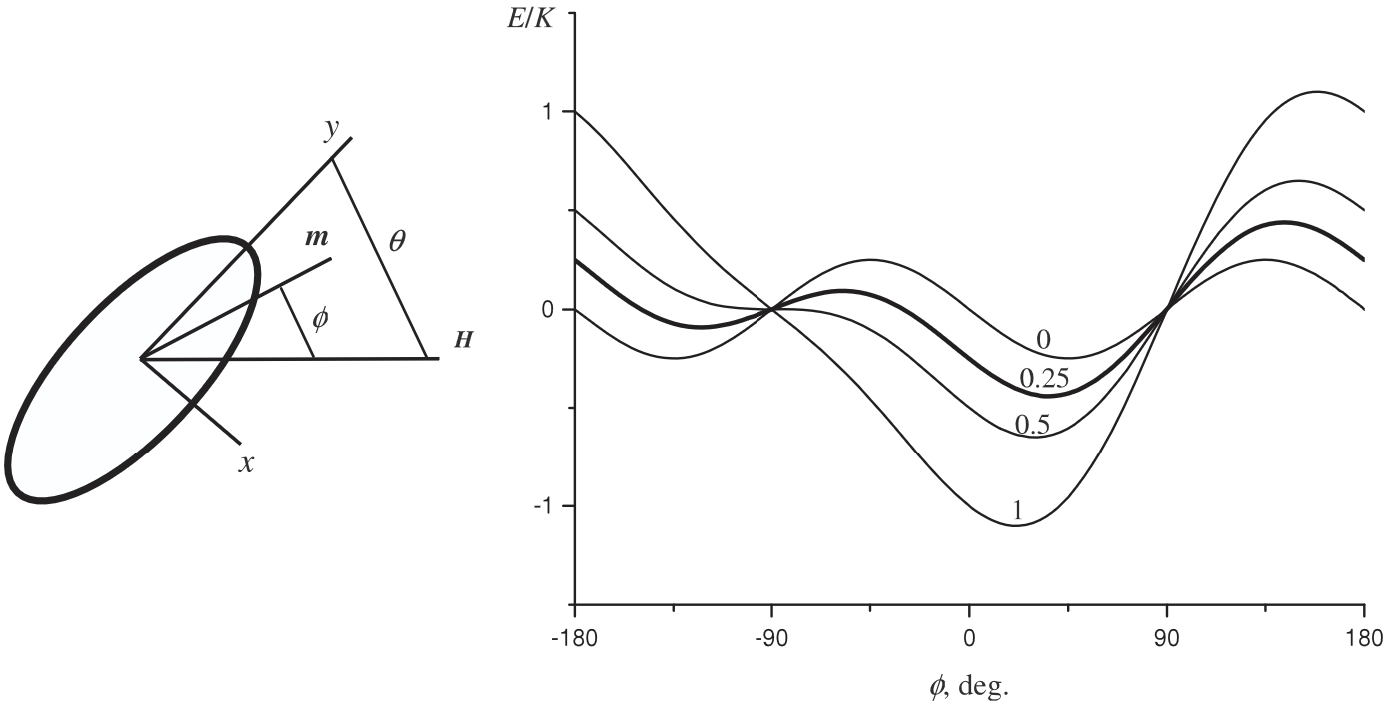
\includegraphics[width=14cm]{./images/SW_Chuev.png}
        \caption{Left: The SW model geometry, where y signifies the magnetic easy axis, H the external magnetic field, $\theta$ the angle between both, m the magnetization of the particle, $\phi$ the angle between m and H and x the magnetic hard axis. Right: An example of resulting energy densities of a SW particle as a function of $\phi$, here with $\theta = 45^\circ$ for different noted field strengths given in multiples of the critical field $H_\mathrm{c}$ over the easy axis. Source: \cite{Chuev2007}.}
        \label{fig_SW}
    \end{center}
\end{figure}

The generalized Stoner-Wohlfarth model (gSW) \cite{Chuev2007} recognizes the possibility  of transitions between minima, especially when the field takes values close to the critical field where the energy barrier between the two minima is low. It therefore differs from SW only for field strength below the critical value.
The probability to transition from the first minimum to the second is derived from the Neel equation \cite{Bean1959}

\begin{equation}
    p_ = p_0 \exp(-U/k_\mathrm{B} T)
    \label{eqn_Neel}
\end{equation}

with fluctuation rate $p_0$, energy barrier U, boltzmann constant $k_\mathrm{B}$ and Temperature T and here takes the form

\begin{equation}
    p_{12}(\theta, H, T) = \frac{p_0}{2} \sum_{i=1,2} \exp\left[-\frac{U_{1i}(\theta, H)}{k_\mathrm{B} T}\right]
    \label{eqn_transition_probability1}
\end{equation}
and vice versa,
\begin{equation}
    p_{21}(\theta, H, T) = \frac{p_0}{2} \sum_{i=1,2} \exp\left[-\frac{U_{2i}(\theta, H)}{k_\mathrm{B} T}\right],
    \label{eqn_transition_probability2}
\end{equation}

$U_{ji}$ being the Energy difference between the i-th maximum $E_i^{(max)}$ and the j-th minimum $E_j^{(min)}$. The sum over both barriers makes this effectively the transition probability over the average energy barrier to better reflect that it lives on a sphere. In the limit of high anisotropy Energy this probabilty goes to zero and reproduces the assumption of the SW model of no transitions.

In accordance with the Boltzmann distribution \cite{Boltzmann2012}, the two relative equilibrium populations of the minima given an ensemble of gSW particles with coaligned easy axes, or equivalently, the probability density of finding a single dipole in the minimum corresponding to $E_j^{(min)}$ are
\begin{equation}
    w_j(\theta,H,T) =
    \frac{ \exp\left[-E_j^{(\min)}(\theta,H)/(k_\mathrm{B} T)\right]}
    {\exp\left[-E_1^{(\min)}(\theta,H)/(k_\mathrm{B} T)\right]+
        \exp\left[-E_2^{(\min)}(\theta,H)/(k_\mathrm{B} T)\right]}.
    \label{eqn_population}
\end{equation}

Together, transition probability and equilibrium population satisfy detailed balance $w_1 p_{12} = w_2 p_{21}$.

The expectation value of the magnetization in direction of the field of an SW particle can be described as the magnetic moment $m_\mathrm{j}$, corresponding to the minimum j and projected onto the field direction, weighed by the equilibrium populations.
\begin{equation}
    m_\mathrm{SW}(\theta,H,T) = w_1(\theta,H,T)m_1(\theta,H) + w_2(\theta,H,T)m_2(\theta,H)
\end{equation}
Here, each of the magnetic moments, $m_\mathrm{SW}, m_1, m_2$, is normalized by $M_\mathrm{sat}$.


\subsection{Initial magnetization of a non-interacting solid}
To do some basic validation of simulation results later, we establish the expected behaviour based on theory here.

The initial equilibrium magnetization m of a larger system of gSW particles, can be obtained by averaging an individual particle's initial magnetization over the distribution of orientations of the constituent particles.

\begin{equation}
    m(H,T) = \int_0^{\pi/2} p(\theta) \sum_{j=1,2}m_\mathrm{j}w_\mathrm{j} \,d\theta,
    \label{eqn_equil}
\end{equation}
integrating only from 0 to $\pi/2$ for symmetry reasons.

\subsubsection{with aligned easy axes}
For a system of gSW particles in which the easy axes are coaligned with the field, $p(\theta) = \delta(\theta)$ and therefore Equation \ref{eqn_equil} can be solved as

\begin{equation}
    m_\mathrm{||}(H,T) = m_1w_1 + m_2w_2 = 1\cdot w_1 -1 \cdot w_2 = \tanh\left[\frac{MH}{k_\mathrm{B}T}\right].
    \label{eqn_tanh}
\end{equation}
For the detailed calculations see Appendix \ref{app:theta_zero}.
\subsubsection{with randomly distributed easy axes}
In a system of gSW particles with randomly, on a sphere, distributed easy axes, where $p(\theta) = \sin \theta$, Equation \ref{eqn_equil} takes the form:

\begin{equation}
    m(H,T) = \int_0^{\pi/2} \sin\theta \sum_{j=1,2}m_\mathrm{j}w_\mathrm{j} \,d\theta,
    \label{eqn_equil_rv}
\end{equation}

which is much less trivial to solve. For validation purposes it is later solved numerically.

\section{Methods}

\subsection{Langevin thermostat}
The usual approach to simulating thermally active particles in molecular dynamics simulations, is to apply a so called thermostat to a system. This isn't necessary for the thermalized magnetic dynamics since they are handled by a dedicated algorithm, but for the purpose of finding ellipsoid geometries thermalized particles will be used to explore possible configurations.

A Langevin thermostat \cite{Allen2017} is an algorithm that implements a canonical NVT ensemble. It discretizes the forces to be used by the integrator, by summing the deterministic forces acting on a particle, and adding additional terms for dampening and diffusion
\begin{equation}
    m_i \dot{\mathbf{v}}_i(t)
    = \mathbf{f}_i(\{\mathbf{x}_j\}, \mathbf{v}_i, t)
    - \gamma \mathbf{v}_i(t)
    + \sqrt{2\gamma k_B T}\,\boldsymbol{\eta}_i(t),
    \label{eqn_therm}
\end{equation}

with velocity $\mathbf{v}$, force $\mathbf{f}$, position $\mathbf{x}$, time t, friction coefficient $\gamma$ and a random "thermal" force $\mathbf{\eta}$ as well as mass m not to be confused with the normalized magnetization m anywhere outside of Chapter 3.1 and 3.2.

\subsection{Velocity Verlet}
To iterate the system, a way to solve its equations of motion is required. The algorithms devised for this purpose are reffered to as integrators in molecular dynamics.

The velocity verlet integrator \cite{Swope1982} is a second order algoritm to integrate Newton's equations of motion, used here, in finding ellipsoid geometries. This specific implementation, has explicit dependence of the force F on velocity, as shown in Equation \ref{eqn_therm}. It is discretized in the following four steps \cite{Rapaport2004}. Calculate the velocity $\mathbf{v}$ at the half step (\ref{eqn_7}), the new position $\mathbf{x}$ (\ref{eqn_8}), the new force $\mathbf{F}$ (\ref{eqn_9}) and then the new velocity $\mathbf{v}$(\ref{eqn_10}). The calculated force at the new position is also saved and reused in the next integration step.

\begin{equation}
    \mathbf{v}(t + \frac{d t}{2}) = \mathbf{v}(t) + \frac{\mathbf{F}(\mathbf{x}(t + d t), \mathbf{v}(t - d t/2),t)}{m}\frac{d t}{2},
    \label{eqn_7}
\end{equation}

\begin{equation}
    \mathbf{x}(t + d t) = \mathbf{x}(t) + \mathbf{v}(t + \frac{d t}{2}) dt,
    \label{eqn_8}
\end{equation}

\begin{equation}
    \mathbf{F}(t + d t) = \mathbf{F}(\mathbf{x}(t + d t), \mathbf{v}(t + \frac{dt}{2}),t + d t),
    \label{eqn_9}
\end{equation}

\begin{equation}
    \mathbf{v}(t + d t) = \mathbf{v}(t + \frac{d t}{2}) + \frac{\mathbf{F}(\mathbf{x}(t + d t), \mathbf{v}(t + d t/2), t + dt)}{m}\frac{d t}{2},
    \label{eqn_10}
\end{equation}

with  time step dt.

\subsection{Finding ellipsoid geometries}
The generation of configurations of raspberry ellipsoids of specifiable sizes and shapes uses physical processes, namely thermalized hard sphere particles, but is entirely haphazardous regarding the sequence in which processes are applied. They merely serve the goal of efficiently finding configurations with convenient properties.

\subsubsection{Smooth shell configurations}
The first implemented approach has a dynamic number of particles it tries to maximize, in a specified size of ellipsoid. It also guarantees a surface that is as densly populated as possible. This is motivated by the intention to have these particles emulate a solid within a solvent.\\
It performs two steps. First, it populates the surface and then the interior defined by the previous step.

A number of particles given by an upper bound estimate for how many will fit are positioned on the surface in a random configuration. They interact via a Weeks-Chandler-Anderson potential. The system is iterated (via velocity Verlet integrator) at very low temperature (using a Langevin thermostat), with the particle positions getting rescaled to the ellipsoid surface after each step.\\
This results in an evenly filled, but tightly packed surface with many overlaps between particles. The mean distance between next neighbours is tracked, as well as the smallest distance between any of those pairs. The target for both is, to reach a value higher than the particle diameter. Once neither metric improves for a set amount of time, a particle is removed, to allow a looser configuration. This is repeated until a configuration is found where no overlap exists anymore and the particles are then fixed in space.\\
There are several optimizations involved, such as setting a higher temperature for a brief time after particle removal to equalize faster, and only checking thoroughly for suitable conafigurations after the tracked values are suitably close to the target.

To fill the interior, another number of particles is positioned inside the ellipsoidal bound, in a hexagonal packing, interacting with each other and the outer shell and then iterated. This leads to strong forces that push particles through the outer shell. After an amount of force indicating particles overlapping strongly is not exceeded for a set time anymore, all particles outside the ellipsoid are removed and the rest continue to try and find a suitable configuration after the same method as detailed for the shell.


\subsubsection{Homogeneous configurations}
In the second implemented approach, a fixed number of particles is placed inside a defined shell and then iterated. The particles' positions are only rescaled to the surface of the ellipsoid if they exceed its boundaries. If no configuration without overlap is found, the dimensions of the ellipsoid are scaled up relative to the remaining overlap between particles. After a successful configuration is found, the ellipsoid is scaled back down to the average size between successful and unsuccessful scale factor, similar to a bisection iteration.

\subsection{Thermal Stoner-Wohlfarth}
The implementation of the gSW used here to simulate the magnetics of the ellipsoids \cite{Mostarac2025} is split in three steps. Finding the extrema in Energy, calculating the energy barrier and determening the transition probability.\\
Speaking more precisely on the latter, the damping time of the Lamor precession $\tau_0$ \cite{Poperechny2014} is used as a time scale to define a modified Neel time \cite{Brown1963} that characterizes the average time it takes a particle to overcome a given energy barrier
\begin{equation}
    \tau_\mathrm{N} = \frac{\tau_0}{2}  \sqrt{\frac{\pi}{\sigma}} \exp(\Delta E \sigma) \quad \text{ with } \quad  \sigma = KV/k_\mathrm{B}T
    \label{eqn_neel_time}
\end{equation}
where V is particle Volume and $\Delta E$ is the lowest energy barrier between minima. This implementation disregards the considerations of the gSW model on the average over energy barriers.

The Neel time is then used to describe the transition probability
\begin{equation}
    p = 1 - \exp(\delta t/\tau_N)
    \label{eqn_trans}
\end{equation}
with $\delta t$, a seperate time step, decoupled from the molecular dynamics time step dt taken in the velocity Verlet algorithm for instance.\\
Then a number is sampled from a uniform distribution between zero and one, and if it is lower than the value of the probability the magnetic moment is flipped to the other minimum.


\newpage
\section{Results and discussion}

For the majority of the simulation results, the molecular dynamics software package ESPResSo \cite{Weeber2024} \cite{Weik2019} \cite{Grad2026} was used.
\subsection{Ellipsoid setup}

The implemented algorithms for the setup of the ellipsoid are capable of any aspect ratio, either at fixed size or fixed particle number. As can be seen in Figure \ref{fig_ell_smooth}, the smooth shell algoritm naturally still produces defects in the surface of the particle, but much less so than the homogenous algorithm, see Figure \ref{fig_ell_hom}.

The smooth shell algorithm, which does the filling of the inside in a second step produces relatively large gaps inside the ellipsoid, especially in thin ones.\\
The homogeneous algorithm performs significantly faster, produces a smooth enough surface to be comparable, and achieves tighter overall packing.\\
For an animation of the homogenous algorithm, refer to \href{https://www.dropbox.com/scl/fi/wk6ookkopgakmzsjxt2yx/Homogenous_algorithm.mp4?rlkey=q6yjftmlc82nsfmpwtvabh9u9&st=u2irjsc7&dl=0}{this link}.

\begin{figure}[H]
    \begin{center}
        
\includegraphics[width=15.5cm]{./images/6_2_2.png}
        \caption{An ellipsoid with semi axes lengths a = 6, b = c = 2, generated by the smooth shell algorithm.}
        \label{fig_ell_smooth}
    \end{center}
\end{figure}


\begin{figure}[H]
    \begin{center}
        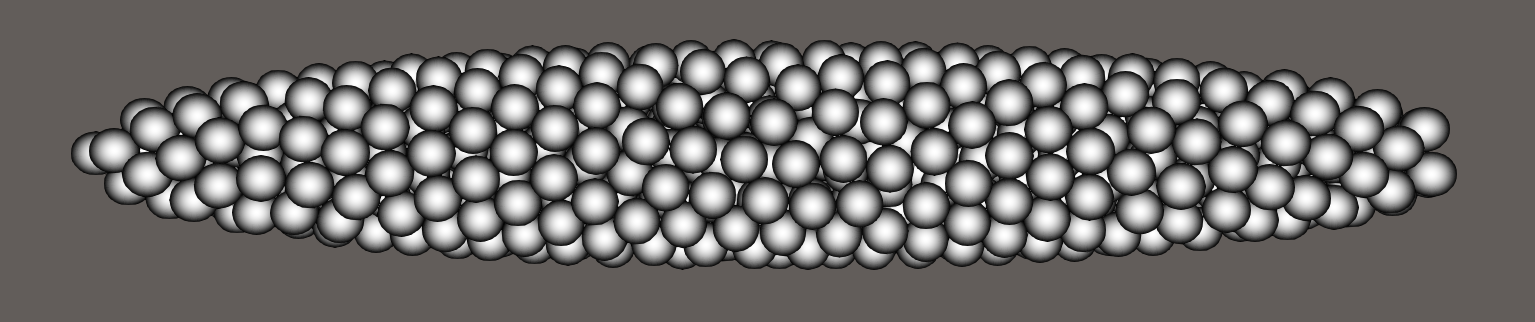
\includegraphics[width=15.5cm]{./images/512_ell.png}
        \caption{An ellipsoid with 512 constituent particles and principal axes ratio 6:1:1 generated by the homogenous algorithm.}
        \label{fig_ell_hom}
    \end{center}
\end{figure}


\subsection{Magnetic properties}

For the discussion of the magnetic behaviour of the constructed ellipsoids, it will be useful to make several clarifications first. Across all results, simulations were carried out with $k_\mathrm{B}T = 1$, diameter d = 1, vacuum permeabilty $\mu_0 = 1$ and mass m = 1. From here on I will refer to field co-aligned easy axes as 'ali' and random easy axes as 'rea'. Let's also define the dipole-dipole interaction parameter
\begin{equation}
    \lambda = \frac{\mu_0 \mu^2}{4\pi d^3 k_\mathrm{B}T}
\end{equation}
where $\mu$ refers to the magnetization of one particle,

the Langevin parameter
\begin{equation}
    \xi = \frac{\mu_0 \mu H}{k_\mathrm{B}T}
\end{equation}

and the anisotropy parameter
\begin{equation}
    \sigma = \frac{K V}{k_\mathrm{B}T}
\end{equation}

each quantifying the strength of an interaction in relation to the thermal energy.

\newpage
\subsubsection{Validation of initial magnetization curve}

The here chosen way to validate the performance of the thermal Stoner Wohlfarth algorithm, is to compare the initial equilibrium magnetization of non-interacting solids of different easy axes distributions to the predictions of the underlying models.\\
The simulation results follow the predictions given by Equations \ref{eqn_tanh} \& \ref{eqn_equil_rv} very nicely, as shown in Figure \ref{fig_model_fit}. Also shown are the results obtained for systems with dipolar interaction enabled. Since the particles are immobilized, we expect the dipolar interaction to demagnetize the system, i.e. lower initial magnetization, which is what can be observed.\\
The solid was aproximated as a 5 by 5 by 5 block of fcc unit cells, where for the interacting systems, two periodic images in each direction were included.

\begin{figure}[H]
    \begin{center}
        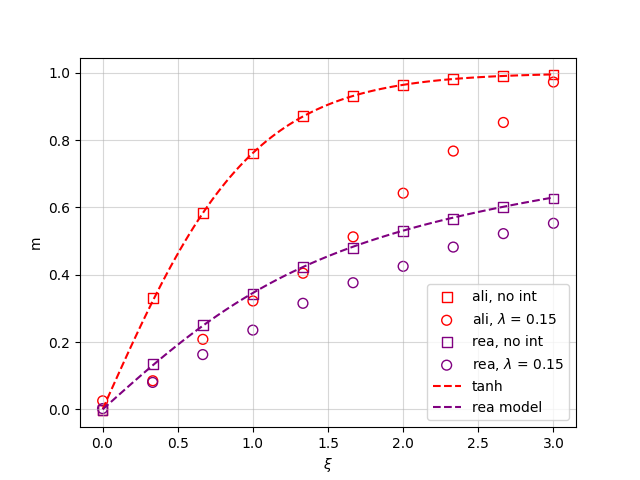
\includegraphics[width=14cm]{./images/Model_fit.png}
        \caption{Magnetization m as a function of the Langevin parameter $\xi$. Initial magnetizaton curves for non-interacting and interacting simulated systems, ones with ali orientation and ones with rea distribution. The functions 'tanh' and 'rea model' correspond to Equations \ref{eqn_equil} \& \ref{eqn_equil_rv}.}
        \label{fig_model_fit}
    \end{center}
\end{figure}

\newpage
\subsubsection{Influence of ellipsoidal geometry on hysteresis}

The relevant properties to the ellipsoids magnetic behaviour are their semi axes ratio r, the orientation of the constituent particles' anisotropy axes and the strength $\sigma$ of the latter.\\
This section shows the influence of each of the parameters on the dynamic hystereses loops of the ellipsoids. All ellipsoid geometries used from here on out were generated using the homogenous algorithm. In all cases the ellipsoids are oriented with their long axis in line with the applied magnetic field. When done in equilibrium the area of all hysteresis loops goes to zero as expected.

For an animation of one hysteresis sweep, reffer to \href{https://www.dropbox.com/scl/fi/klkqul893hg7puq5soq2m/Hysteresis.mp4?rlkey=0k68552s0b20lvw52iaiftr1p&st=2bwjdtpg&dl=0}{this link}. It shows the exact system for r = 2 in Figure \ref{fig_ratio_hyst}.

The ellipsoids, both rea and ali, exhibit hystereses that are more square than an interacting solid system. That is, they show higher remanence $m_\mathrm{r}$ at zero field, post saturation, as well as coercive field $H_\mathrm{c}$. More so for the system with ali orientation, since in that case full alignment of the magnetization with the field minimizes the anisotropy energy term. See Figure \ref{fig_geom_hyst}.

The strength of the dipole interaction $\lambda$ correlates inversely to the slope of the hysteresis. Generally speaking the dipole interaction demagnetizes after all. For some parameter combinations, rising $\lambda$ also extends the time for which peak magnetization is held since it encourages chain formation, increasing coercivity. See Figure \ref{fig_lambda_hyst}.

In some cases, with rea distribution, for small enough easy axes ratio, that is, relatively spherical ellipsoids, demagnetization effects visibly kick in, while still retaining saturation magnetization for relatively long. This leads to hourglass shaped hystereses loops.\\
Generally, as one of the core observations, under rea distribution, where there is no inherent net anisotropy due to the constituent particles' easy axes, hystereses squareness still goes up with semi axes ratio r. This indicates the emergent shape anisotropy of the ellipsoids independent of the anisotropy of each individual particle. The thinner the ellipsoid the more energetically stable become the chain formations that satisfy the dipole interaction. For both of these observations refer to Figure \ref{fig_ratio_hyst}.

With rea distribution, $\sigma$ lessens net anisotropy and with it squareness of the hysteresis. When the easy axes are aligned with the ellipisoid, $\sigma$ obviously enhances net anisotropy instead. See Figure \ref{fig_KV_hyst}.

\begin{figure}[H]
    \begin{center}
        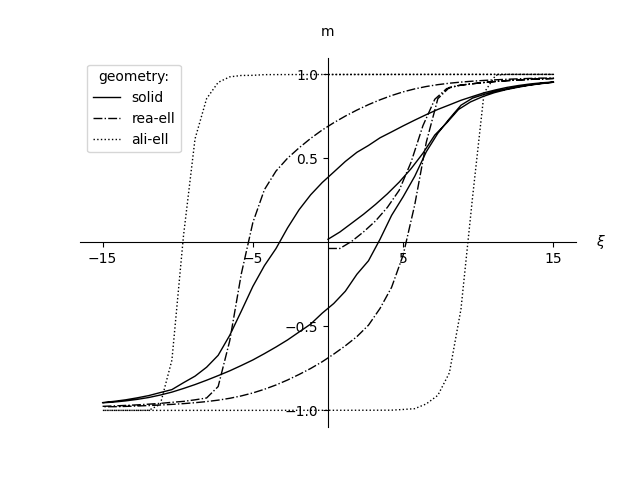
\includegraphics[width=11cm]{./images/1_solid_vs_ell_rea_vs_zani.png}
        \caption{Magnetization m as a function of the Langevin parameter $\xi$. Comparison of the hystereses of a solid, an ellipsoid with randeom easy axes distribution (rea) and an ellipsoid with field aligned (ali) easy axes. For all three systems $\lambda = 0.2$ and $\sigma$ = 5. The ellipsoids have a semi axes ratio of r = 6.}
        \label{fig_geom_hyst}
    \end{center}
\end{figure}
\vspace{-0.5cm}
\begin{figure}[H]
    \begin{center}
        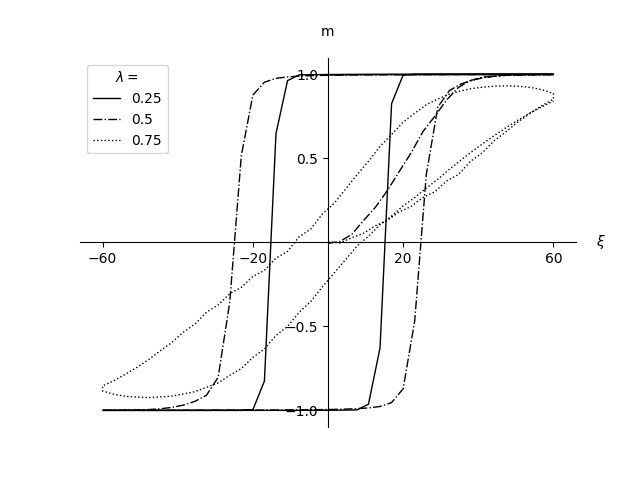
\includegraphics[width=11cm]{./images/2_lambda_zani.png}
        \caption{Magnetization m as a function of the Langevin parameter $\xi$. Comparison of the hystereses of ellipsoids with three different values for the dipolar interaction strength $\lambda$. For all three r = 6, $\sigma$ = 5 and ali distribution.}
        \label{fig_lambda_hyst}
    \end{center}
\end{figure}

\begin{figure}[H]
    \begin{center}
        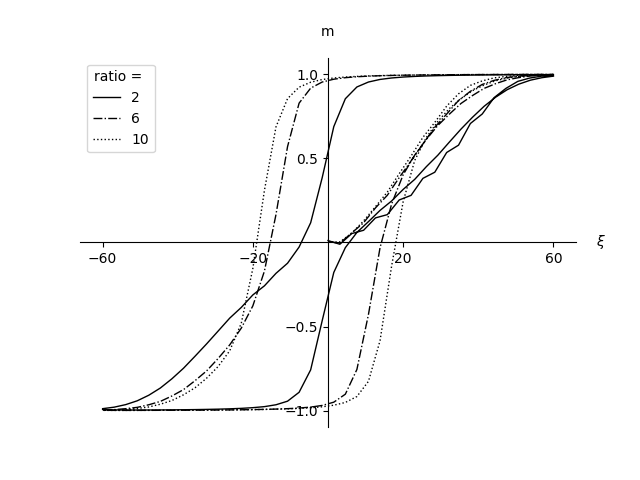
\includegraphics[width=11cm]{./images/3_ratio_rea.png}
        \caption{Magnetization m as a function of the Langevin parameter $\xi$. Comparison of the hystereses of ellipsoids with different easy axes ratios r. For all three systems $\sigma$ = 5, $\lambda = 0.5$ and rea distribution.}
        \label{fig_ratio_hyst}
    \end{center}
\end{figure}

\begin{figure}[H]
    \begin{center}
        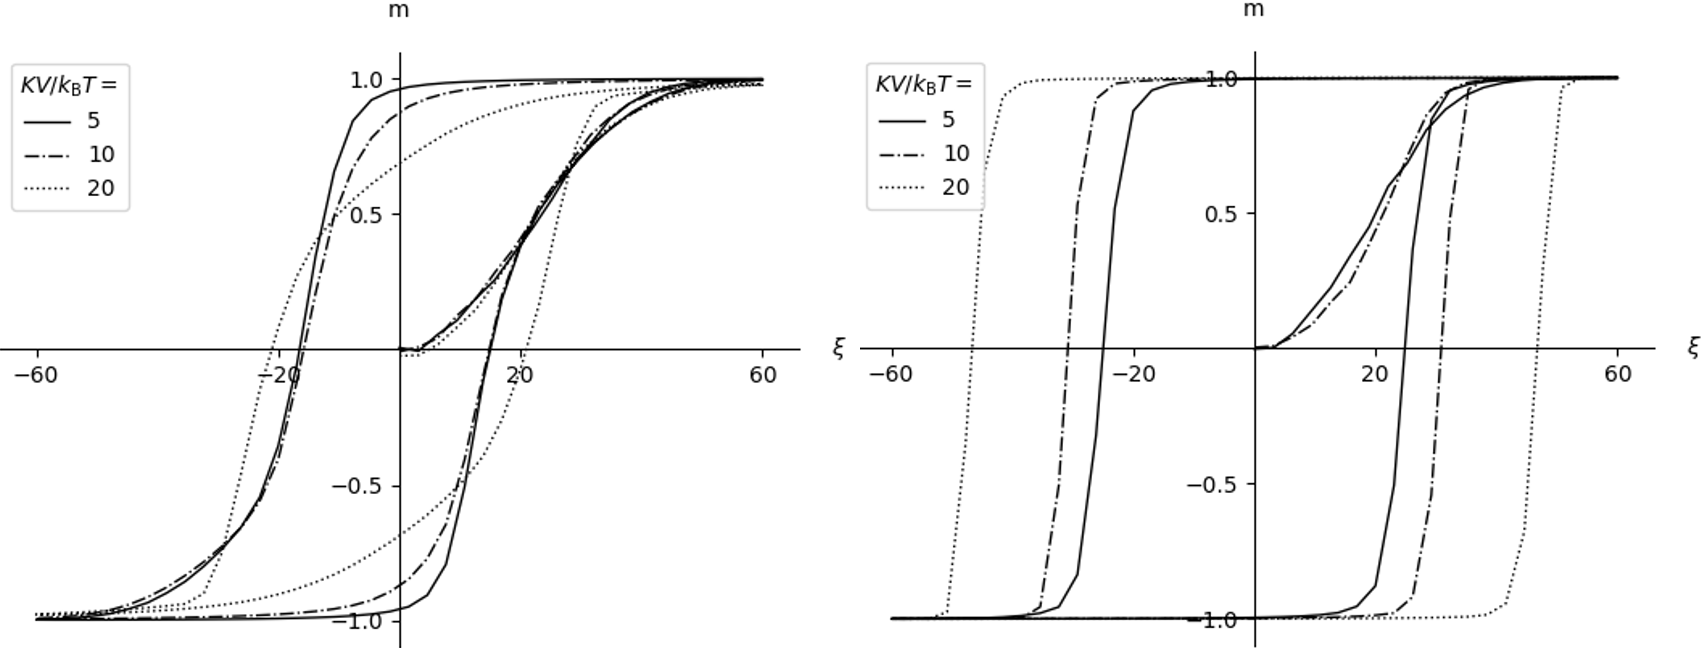
\includegraphics[width=15cm]{./images/4_KV_rea_vs_zani.png}
        \caption{Magnetization m as a function of the Langevin parameter $\xi$. Comparison of the hystereses of ellipsoids with different anisotropy stregths $\sigma$ with rea distribution (left) and with ali orientation (right). For all systems r = 6 and $\lambda = 0.5$.}
        \label{fig_KV_hyst}
    \end{center}
\end{figure}

\section{Conclusion}
\subsection{Summary of findings}
The creation algorithms for the ellipsoid geometries work well enough for their intended purpose, but there are serious flaws in the chosen approach.\\
Despite a good amount of time spent optimizing, they remain gruelingly inefficient due to the poor conditioning of the problem. The nature of the WCA potential in combination with the number of neighbour pairs leads to massive amounts of computational time being wasted on persistent, tiny overlaps.\\
In the homogeneous algorithm, where the boundary of the ellipsoid grows, the system needs to be able to push another particle into the surface layer, for which it is necessary to disturb many already settled, close packed particles.\\
In hindsight it might be most practical to completely shuffle the system after increasing the scale of the ellipsoid to completely leave behind the established configuration.

Non-interacting magnetic systems match expected equilibrium behaviour very well.
All explored parameters produce the qualitatively expected results on hystereses as well as some unforseen ones for specific parameter combinations.\\
Generally, the system seems surprisingly sensitive to the dipolar interaction strength. This may be due to finite size effects associated with the ellipsoidal geometry, but might also have arisen from some mishap with parameter scaling.

\subsection{Outlook}
The thermal Stoner-Wohlfarth method should serve well as a tool for further simulation, altough the specific demands for that are not yet exactly clear. It does brings with it the limitation, that for raspberry particles which are free to rotate, the configuration of easy axes will be limited to homogenous across the entire ellipsoid, which will effectively mean in line with its principal axis, as having a net anisotropy along any other axis will be unlikely to make sense. This shouldn't pose a great hindrance all things considered.

Further work to be done includes, in order, specifying unit scales to work roughly in accordance with the source paper, exploring the response to rotating magnetic field, implementing fluid dynamics, setting up the experiment geometry and finally trying to recreate the recirculation flows.


\newpage
\appendix
\section*{Appendix}
\addcontentsline{toc}{section}{Appendix}
\section{Equilibrium magnetization calculations}
\label{app:theta_zero}
\[
    \text{with Equations \ref{eqn_ani} and \ref{eqn_zee} as well as }\qquad \theta=0\Longrightarrow\phi_1=0,\quad\phi_2=\pi
\]
\[
    \text{follows } E_1=-K-MH,\qquad E_2=-K+MH
\]

\[
    m_{||}(H,T)=\frac{e^{-E_1/(k_{\mathrm B}T)}-e^{-E_2/(k_{\mathrm B}T)}}{e^{-E_1/(k_{\mathrm B}T)}+e^{-E_2/(k_{\mathrm B}T)}}
    =\frac{e^{(K+MH)/(k_{\mathrm B}T)}-e^{(K-MH)/(k_{\mathrm B}T)}}{e^{(K+MH)/(k_{\mathrm B}T)}+e^{(K-MH)/(k_{\mathrm B}T)}}
\]
\[
    =\frac{e^{MH/(k_{\mathrm B}T)}-e^{-MH/(k_{\mathrm B}T)}}{e^{MH/(k_{\mathrm B}T)}+e^{-MH/(k_{\mathrm B}T)}}
    =\boxed{\tanh\!\left(\frac{MH}{k_{\mathrm B}T}\right)}
\]

% ------------------------------------------------------------
\newpage
\bibliographystyle{IEEEtr}
\bibliography{references}

% ------------------------------------------------------------

\end{document}